\chapter{Реализация и экспериментальная проверка работоспособности
модуля}

\section{Реализация парсера terraform plugins}

Для реализации парсера плагинов Terraform был использован язык программирования
Go, так как Terraform написан на этом языке, и большинство его плагинов также
написаны на Go.

Парсер плагинов Terraform реализован как отдельное приложение на Go, которое
анализирует исходный код плагинов Terraform и извлекает из него метаданные,
необходимые для генерации case classes на Scala.

В основе парсера лежит рефлексия, механизм, позволяющий программам исследовать
структуру кода во время выполнения. С помощью рефлексии парсер анализирует
структуру плагина Terraform, извлекает информацию о типах ресурсов и их
свойствах, и преобразует эту информацию в формат, подходящий для генерации case
classes на Scala.

В процессе анализа парсер обходит все структуры и поля в плагине, обрабатывая
каждое поле в зависимости от его типа. Для структур и словарей (map) парсер
рекурсивно обходит их поля, для списков (slice) - их элементы. Функции и другие
необрабатываемые типы пропускаются.

Результат работы парсера - JSON-файл с метаданными плагина, который затем
используется модулем Case Classes Generator для генерации case classes на Scala.

Код парсера находится в Приложении \ref{sec:appendix1}

В этом коде функции walkStruct, walkSlice и walkMap используются для обхода
структур, списков и словарей соответственно. Они вызывают функцию processValue
для каждого поля или элемента, которая в свою очередь обрабатывает значение в
зависимости от его типа и возвращает его в формате, подходящем для записи в
JSON.

Функция valueIsValid используется для определения, является ли значение
обрабатываемым. Она возвращает false для функций и других типов значений,
которые не могут быть корректно преобразованы в JSON.

В функции main происходит инициализация плагина Terraform, извлечение информации
о провайдере с помощью рефлексии, преобразование этой информации в JSON и запись
JSON в файл.

Пример JSON-файла с метаданными плагина Terraform 
см. в Приложении \ref{sec:appendix2}.

Таким образом, парсер плагинов Terraform позволяет извлечь из плагинов
метаданные, необходимые для генерации case classes на Scala. Эти метаданные
включают в себя информацию о типах ресурсов и их свойствах, которые затем
используются при генерации кода на Scala.

\section{Реализация парсера документации}

Парсер документации реализован на языке Python и использует библиотеки json, os,
re и hcl. Он проходит через все файлы в указанной директории, извлекает блоки
кода HCL из файлов с расширением .md или .markdown, парсит их и сохраняет
результат в формате JSON.

Вот основные шаги работы парсера:


\begin{itemize}
  \item Извлечение блоков кода HCL из файлов документации. Это достигается с
помощью функции $extract\_code\_blocks\_from\_directory$, которая проходит через
все
файлы в указанной директории и вызывает функцию
$extract\_code\_blocks\_from\_file$
для каждого файла. Функция $extract\_code\_blocks\_from\_file$ открывает файл,
читает
его содержимое и использует регулярное выражение для поиска блоков кода HCL.
  \item Парсинг блоков кода HCL. Это делается с помощью функции
$parse\_terraform$,
которая принимает на вход массив блоков кода HCL и пытается распарсить каждый из
них с помощью библиотеки hcl. Если парсинг проходит успешно, результат
добавляется в массив $hcl\_arr$.
  \item Преобразование сложных структур данных в плоский формат. Это делается с
помощью функции $flatten\_dict$, которая принимает на вход словарь и преобразует
его в плоский формат, где каждый ключ представляет собой путь к соответствующему
значению в исходном словаре.
  \item Сохранение результатов в файл. После обработки всех блоков кода HCL
результаты сохраняются в файл в формате JSON.
\end{itemize}

Полный код парсера представлен в Приложении \ref{sec:appendix3}.

Пример JSON-файла с метаданными документации Terraform см. в Приложении
\ref{sec:appendix4}.

  \section{Реализация модуля Case Classes Generator}

  Модель состоит из многих файлов, опишем основные из них в текущем разделе.

  \subsection{Реализация Docs Parser}

  Модуль Docs Parser отвечает за обработку и анализ JSON-документации,
полученной
  из Terraform. Он использует библиотеку Circe для декодирования JSON и
библиотеку
  Scala для работы с регулярными выражениями и файлами.

  Вот основные компоненты этого модуля:

  \begin{itemize}
    \item JsonValue: это абстрактный класс, представляющий значение JSON. Он
имеет
  четыре
  подкласса: JsonString, JsonBool, JsonLong и JsonDouble, которые представляют
  соответствующие типы данных JSON.

    \item JsonMap: это тип для представления карты JSON, где ключи - это строки,
а
  значения - это списки значений JSON.

    \item DocsInfo: это класс, который содержит информацию, извлеченную из
  документации.
  Он содержит различные карты для хранения доменов, IP-адресов, масок IP, строк
  JSON и ссылок на поля.

    \item decodeJsonMap: эта функция декодирует строку JSON в JsonMap. Если
  происходит
  ошибка декодирования, она выбрасывает исключение.

    \item filterJsonMap: эта функция фильтрует JsonMap, оставляя только ключи,
  которые
  начинаются с "output.", "resource." или "data.".

    \item definePatterns: эта функция определяет регулярные выражения для
  различных типов
  значений, таких как поля, домены, IP-адреса и маски IP.

    \item decodeAndFilterJson: это основная функция модуля. Она принимает строку
  JSON,
  декодирует ее в JsonMap, фильтрует карту, извлекает различные типы значений и
  возвращает DocsInfo с этой информацией.
  \end{itemize}


  \subsection{Описание классов и функций}

  Основные классы представлены на рисунке \ref{fig:uml1}.

  \begin{figure}[h]
    \centering
    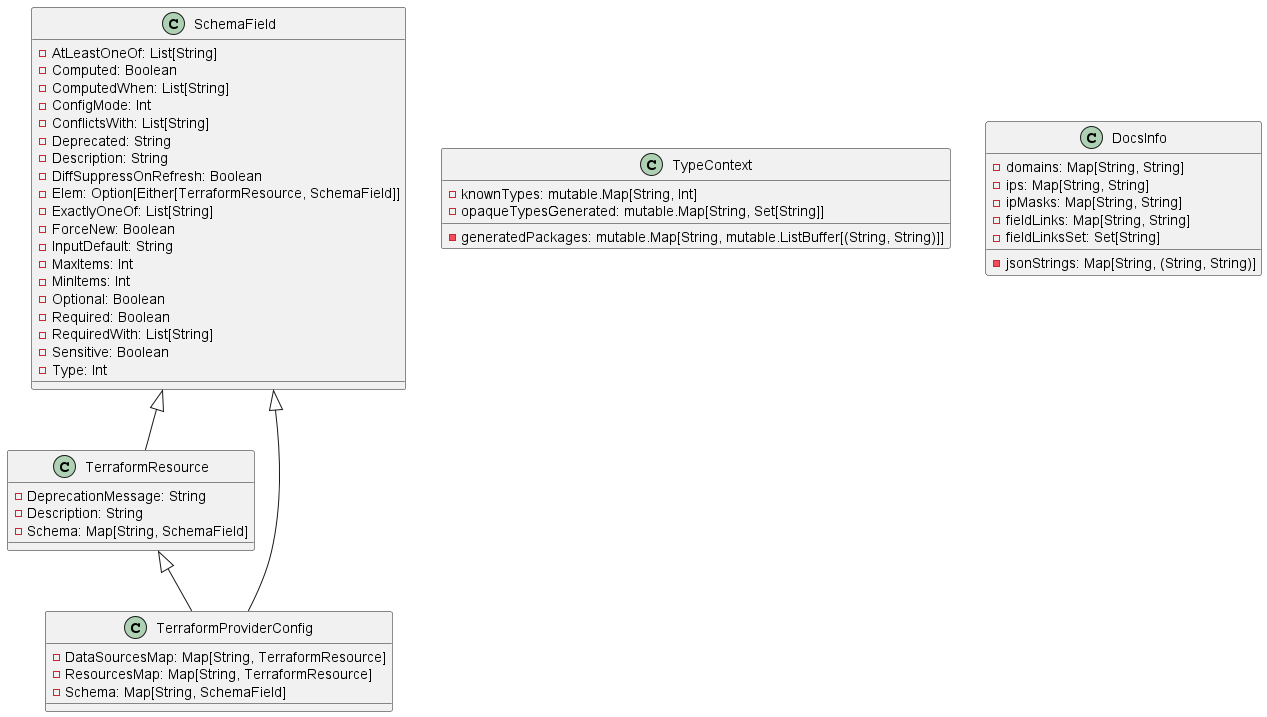
\includegraphics[scale=0.35]{img/5.png}
    \caption{Основные классы модуля Case Classes Generator}
    \label{fig:uml1}
  \end{figure}

  \vspace{60mm}

  Далее опишем основные классы и функции модуля.

  

  \begin{itemize}
    \item $SchemaField$: Этот класс представляет собой модель для полей схемы в
  Terraform. Он содержит различные атрибуты, такие как $AtLeastOneOf$,
$Computed$,
  $ComputedWhen$, $ConfigMode$, $ConflictsWith$, $Deprecated$, $Description$,
  $DiffSuppressOnRefresh$, $Elem$, $ExactlyOneOf$, $ForceNew$, $InputDefault$,
  $MaxItems$, $MinItems$, $Optional$, $Required$, $RequiredWith$, $Sensitive$,
  $Type$. $Elem$ - это опциональное поле, которое может содержать либо
  $TerraformResource$, либо другой $SchemaField$.

    \item $TerraformProviderConfig$: Этот класс представляет конфигурацию
  провайдера Terraform. Он содержит карты для $DataSourcesMap$, $ResourcesMap$ и
  $Schema$.

    \item $TerraformResource$: Этот класс представляет ресурс в Terraform. Он
  содержит \newline $DeprecationMessage$, $Description$ и $Schema$.

    \item $TypeContext$: Этот класс содержит контекст для типов, включая
  $knownTypes$, $generatedPackages$ и $opaqueTypesGenerated$.

    \item $DocsInfo$: Этот класс содержит информацию, извлеченную из
документации
  Terraform. Он содержит карты для $domains$, $ips$, $ipMasks$, $jsonStrings$,
  $fieldLinks$ и множество $fieldLinksSet$.

    \item $TypeCodes$: Этот объект содержит константы для различных типов полей.

    \item $TypeContext$: Этот класс содержит контекст для типов, включая
  $knownTypes$, \newline $generatedPackages$ и $opaqueTypesGenerated$.

    \item $generateFieldType$: Эта функция генерирует тип поля на основе
  $SchemaField$.

    \item $updateFieldWithType$: Эта функция обновляет поле с типом на основе
  $SchemaField$.

    \item $generateTodoComment$: Эта функция генерирует комментарий TODO для
поля.

    \item $generateSchemaForElem$: Эта функция генерирует схему для элемента на
  основе  \newline $SchemaField$.

    \item $generateSchemaField$: Эта функция генерирует поле схемы на основе
  $SchemaField$.

    \item $generateResourceClassName$: Эта функция генерирует имя класса
ресурса.

    \item $generatePackageName$: Эта функция генерирует имя пакета.

    \item $generateFullName$: Эта функция генерирует полное имя.

    \item $generateFields$: Эта функция генерирует поля для ресурса.

    \item $getUniqueClassName$: Эта функция генерирует уникальное имя класса.

    \item $generateToHCLBody$: Эта функция генерирует тело метода toHCL.

    \item $generateToHCLMethod$: Эта функция генерирует метод toHCL.

    \item $generateFieldDescriptions$: Эта функция генерирует описания полей для
  ScalaDoc.

    \item $generateClassDoc$: Эта функция генерирует документацию для класса,
  включая описание ресурса и описания полей.

    \item $generateDeprecationAnnotation$: Эта функция генерирует аннотацию
  устаревания, если ресурс устарел.

    \item $generateClassDef$: Эта функция генерирует определение класса, включая
  его поля и методы.

    \item $generatePackageCode$: Эта функция генерирует код пакета, включая
  определения классов и связанных полей.

    \item $updateContext$: Эта функция обновляет контекст, добавляя новые классы
и
  пакеты.

    \item $generateLinkedFields$: Эта функция генерирует связанные поля для
  ресурса.

    \item $generateResourceClass$: Эта функция генерирует класс ресурса на
основе
  конфигурации ресурса.

    \item $generateCaseClasses$: Эта функция генерирует классы case для
  конфигурации провайдера.

    \item $generateDataSources$: Эта функция генерирует исходные данные для
  конфигурации провайдера.

    \item $generateResources$: Эта функция генерирует ресурсы для конфигурации
  провайдера.

    \item $generateProviderResource$: Эта функция генерирует ресурс провайдера
для
  конфигурации провайдера.

    \item $printFieldLinksInfo$: Эта функция выводит информацию о связанных
полях.

    \item $generatePackages$: Эта функция генерирует пакеты на основе контекста.

    \item $generateProviderPackage$: Эта функция генерирует пакет провайдера.
  \end{itemize}


Код для данного модуля не будет приведен в текущей статье из-за его большого
объема. Полный код доступен в репозитории проекта.

\subsection{Пример работы}

В этом примере мы используем библиотеку Circe для декодирования JSON,
представляющего конфигурацию провайдера Terraform, и генерируем соответствующие
классы Scala.

Сначала мы читаем JSON из файла и декодируем его в объект
TerraformProviderConfig. Затем мы генерируем классы Scala для каждого ресурса и
источника данных в конфигурации провайдера с использованием функции
generateCaseClasses. Наконец, мы записываем сгенерированный код Scala в файлы в
соответствующих пакетах.

Пример кода см. в Приложении \ref{sec:appendix6}.

Диаграмма классов для сгенерированного кода Scala представлена на рисунке
\ref{fig:uml2}.

\begin{figure}[h]
  \centering
  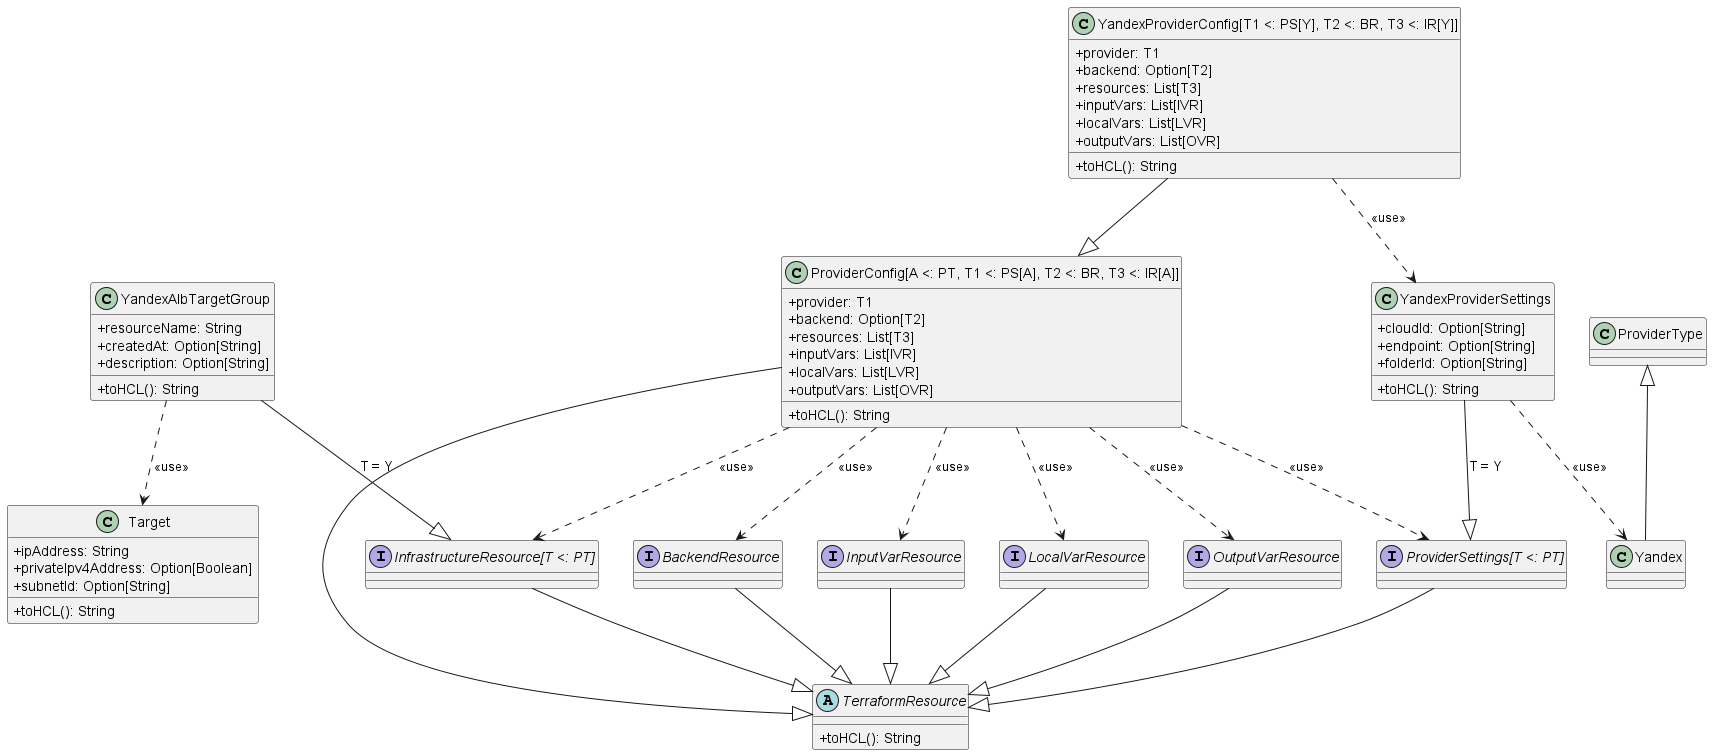
\includegraphics[scale=0.25]{img/6.png}
  \caption{Диаграмма классов для сгенерированного кода Scala}
  \label{fig:uml2}
\end{figure}

В этом примере мы используем файлы JSON, сгенерированные с помощью инструментов
terraform-docs-extractor и terraform-to-json, для представления конфигурации
провайдера Terraform и связанных с ним документов. Эти файлы затем используются
для генерации классов Scala, которые могут быть использованы для работы с этим
провайдером в Scala.

\section{Реализация модуля для работы с Kubernetes API}
\subsection{Описание классов}

В данном модуле определены следующие классы:

\begin{itemize}
\item \textbf{AllocatedResources}: Этот класс представляет выделенные ресурсы.
Он содержит следующие поля: cpuRequests, cpuLimits, memoryRequests,
memoryLimits, ephemeralStorageRequests, ephemeralStorageLimits,
hugepages2MiRequests, hugepages2MiLimits, hugepages1GiRequests,
hugepages1GiLimits. Все поля имеют тип BigDecimal.

\item \textbf{ContainerStates}: Этот класс представляет состояния контейнера. Он
содержит одно поле: id (тип String).

\item \textbf{PodConditions}: Этот класс представляет условия пода. Он содержит
следующие поля: conditionType (тип String) и status (тип Boolean).

\item \textbf{MyPod}: Этот класс представляет под. Он содержит следующие поля:
ip (тип Option[String]), name (тип String), status (тип Option[String]),
startedAt (тип Option[String]), createdAt (тип Option[String]), age (тип
Option[String]), ageInSec (тип Long), restarts (тип Int), states (тип
List[ContainerStates]), allocatedResources (тип AllocatedResources), namespace
(тип String), isSystem (тип Boolean), failedScheduling (тип Boolean), events
(тип Map[String, MyEvent]), conditions (тип List[PodConditions]), uid (тип
String).

\item \textbf{MyNode}: Этот класс представляет узел. Он содержит следующие поля:
name (тип String), status (тип Map[String, Boolean]), pods (тип Map[String,
MyPod]), ip (тип Map[String, String]), allocatedResources (тип
AllocatedResources), capacity (тип Map[String, BigDecimal]), allocatable (тип
Map[String, BigDecimal]), uid (тип String).

\item \textbf{KuberInfo}: Этот класс представляет информацию о кластере
Kubernetes. Он содержит следующие поля: nodes (тип Map[String, MyNode]),
podsWithoutNode (тип Map[String, MyPod]), unscheduledPods (тип Map[String,
MyPod]), events (тип List[MyEvent]), namespaces (тип Set[String]).
\end{itemize}



Uml диаграмма для классов представлена на рисунке \ref{fig:uml3}.
\begin{figure}[h]
  \centering
  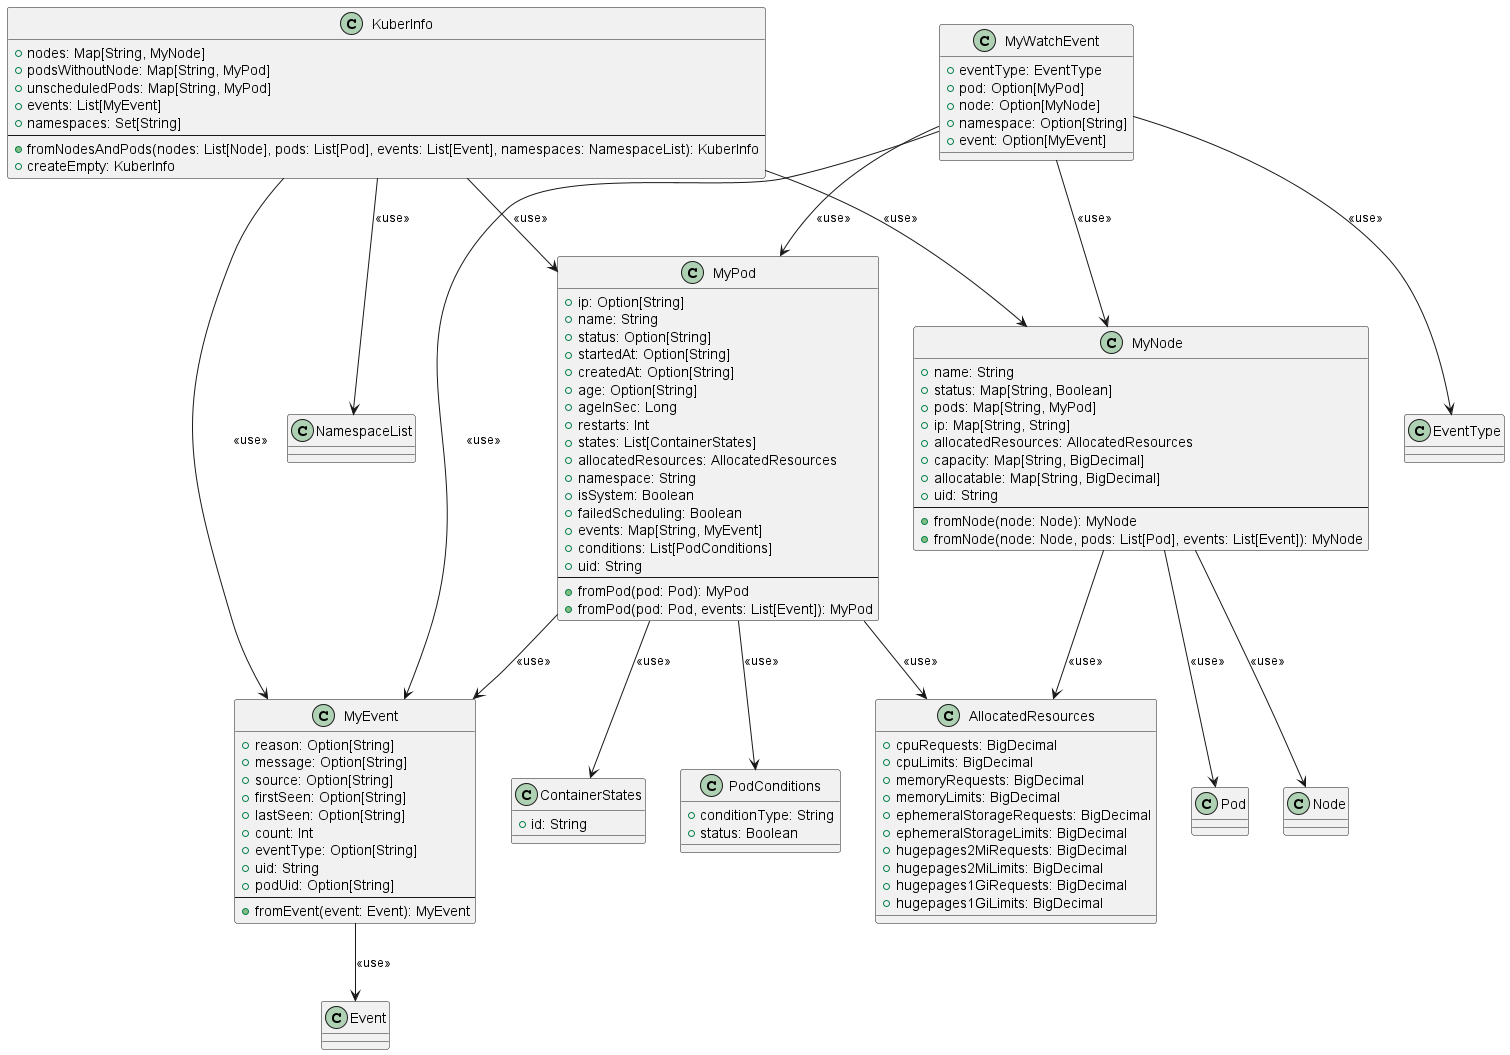
\includegraphics[scale=0.3]{img/7.png}
  \caption{Диаграмма классов модуля Autoscaler}
  \label{fig:uml3}
\end{figure}

\subsection{Описание методов}

\begin{itemize}

\item \textbf{waitUntilAllPodsVerified}: Этот метод ожидает, пока все поды не
будут проверены. Он принимает следующие параметры: statefulSets (тип
List[StatefulSet]), deployments (тип List[Deployment]), replicaSets (тип
List[ReplicaSet]), pollInterval (тип FiniteDuration, по умолчанию 1 секунда),
timeout (тип FiniteDuration, по умолчанию 5 минут), checkRunning (тип Boolean,
по умолчанию true).

\item \textbf{increaseReplicas}: Этот метод увеличивает количество реплик. Он
принимает следующие параметры: resource (тип T, где T является подтипом
ObjectResource), increment (тип Int).

\item \textbf{cordonNode}: Этот метод блокирует узел. Он принимает следующий
параметр: nodeName (тип String).

\item \textbf{getResources}: Этот метод получает ресурсы.

\item \textbf{getAutoscaler}: Этот метод получает автомасштабировщик. Он
принимает следующие параметры: namespace (тип String), deploymentName (тип
String).

\item \textbf{disableAutoscaler}: Этот метод отключает автомасштабировщик. Он
принимает следующие параметры: namespace (тип String), deploymentName (тип
String).

\item \textbf{enableAutoscaler}: Этот метод включает автомасштабировщик. Он
принимает следующий параметр: hpa (тип HorizontalPodAutoscaler).

\item \textbf{deletePod}: Этот метод удаляет под. Он принимает следующие
параметры: pod (тип Pod), gracePeriod (тип Int).

\item \textbf{processResources}: Этот метод обрабатывает ресурсы. Он принимает
следующие параметры: resources (тип List[T], где T является подтипом
ObjectResource), nodePods (тип List[Pod]), deploymentNames (тип
List[Option[String]], по умолчанию пустой список).

\item \textbf{drainNodes}: Этот метод освобождает узлы. Он принимает следующие
параметры: nodeNames (тип List[String]), gracePeriod (тип Int).

\end{itemize}


\section{Создание абстрактного интерфейса для Rustack и Яндекс облака}
Для обеспечения генерации конфигураций Terraform для разных провайдеров (Yandex
и Rustack), мы определяем абстрактный интерфейс и конкретные реализации для
каждого провайдера.

\begin{minted}{Scala}
trait TerraformConfigGenerator[P] {
  def generateClusterConfig(
    servers: Seq[Server],
    masterNode: Option[Server]):
String
}
\end{minted}

\subsection{Определение Сервера}
Тип \texttt{Server} теперь включает флаг для master ноды.

\begin{minted}{Scala}
case class Server(
  cores: Int,
  memory: Int,
  storageSize: Int,
  providerType: ProviderType,
  isMaster: Boolean = false
)
\end{minted}

\subsection{Тип Провайдера}
Перечисление для различных типов провайдеров.

\begin{minted}{Scala}
enum ProviderType {
  case Yandex, Rustack
}
\end{minted}

\subsection{Реализация для Yandex}
Конкретная реализация для Yandex.

\begin{minted}{Scala}
class YandexConfigGenerator extends
TerraformConfigGenerator[ProviderType.Yandex.type] {
  override def generateClusterConfig(
    servers: Seq[Server], 
    masterNode: Option[Server]):
    String = {
    // Логика генерации конфигурации кластера для Yandex
  }
}
\end{minted}

\subsection{Реализация для Rustack}
Конкретная реализация для Rustack.

\begin{minted}{Scala}
class RustackConfigGenerator extends
TerraformConfigGenerator[ProviderType.Rustack.type] {
  override def generateClusterConfig(
    servers: Seq[Server],
    masterNode: Option[Server]):
    String = {
    // Логика генерации конфигурации кластера для Rustack
  }
}
\end{minted}

\subsection{Использование Абстракции}
Пример использования абстракции для генерации конфигурации кластера.

\begin{minted}{Scala}
  val servers = Seq(
    Server(4, 16, 100, ProviderType.Yandex, isMaster = true),
    Server(2, 8, 50, ProviderType.Yandex)
  )
  val configGenerator: 
  TerraformConfigGenerator[ProviderType.Yandex.type] = 
  new YandexConfigGenerator()
  val yandexClusterConfig = 
  configGenerator.generateClusterConfig(servers,
  servers.find(_.isMaster))
  
  // Аналогично для Rustack
\end{minted}

\section{Создание системы автомасштабирования}

В этом разделе описывается, как была реализована система автомасштабирования,
объединяющая HCL генератор (с его абстракцией) и модуль автоскейлинга
Kubernetes.

\subsection{Объединение HCL генератора с модулем автоскейлинга Kubernetes}

Абстракция над HCL генератором позволяет генерировать конфигурации для различных
облачных провайдеров, таких как Yandex и Rustack. Для поддержки
автомасштабирования в Kubernetes, мы расширили эту абстракцию, включив в неё
возможность определения параметров для создания и управления ресурсами
Kubernetes, включая настройку Horizontal Pod Autoscaler (HPA).

\subsubsection{Интеграция с Kubernetes API}

Для взаимодействия с Kubernetes API был разработан отдельный модуль на Scala,
который предоставляет функционал для управления ресурсами кластера, включая
создание и удаление подов, узлов и автомасштабировщиков. Этот модуль включает в
себя различные классы и методы, такие как increaseReplicas, cordonNode,
getAutoscaler и другие.

\subsubsection{Автомасштабирование}

Система автомасштабирования была настроена для мониторинга загрузки CPU и памяти
подов в кластере. При достижении определённых порогов загрузки, модуль
Kubernetes API активирует HPA для автоматического увеличения или уменьшения
количества подов в соответствии с текущими потребностями. Это обеспечивает
эффективное распределение ресурсов и оптимизацию работы приложений.

\subsubsection{Генерация Terraform конфигурации}

HCL генератор использует данные из модуля Kubernetes для создания конфигураций
Terraform, соответствующих текущему состоянию и требованиям кластера Kubernetes.
Например, если система автомасштабирования решает, что необходимо больше
ресурсов, HCL генератор автоматически создаёт и применяет соответствующие
изменения в конфигурации Terraform для обеспечения дополнительных ресурсов в
облаке.

\subsection{Пример работы системы}

Предположим, что в кластере Kubernetes наблюдается высокая загрузка CPU. Система
автомасштабирования определяет необходимость увеличения количества подов для
одного из микросервисов. Эта информация передаётся в HCL генератор, который
генерирует и применяет соответствующие изменения в конфигурации Terraform для
запуска дополнительных экземпляров подов в облачной среде.

Этот процесс обеспечивает гибкое и динамическое управление ресурсами, позволяя
системе масштабироваться в соответствии с текущими потребностями, обеспечивая
при этом оптимальную производительность и стабильность работы приложений.

\section{Выводы}

Созданная система автомасштабирования объединяет в себе гибкость абстракции над
HCL генератором и эффективность модуля автоскейлинга Kubernetes, обеспечивая тем
самым удобное и мощное решение для управления инфраструктурой и ресурсами в
облачных средах.